\documentclass[conference]{IEEEtran}
\usepackage{amsmath}
\usepackage{amssymb}
\usepackage{graphicx}
\usepackage{booktabs}
\usepackage{multirow}
\usepackage{array}
\usepackage{cite}
\usepackage{url}
\usepackage[hidelinks]{hyperref}
\usepackage{xcolor}
\usepackage{tikz}
\usetikzlibrary{arrows.meta,calc,positioning}
\definecolor{pnavy}{HTML}{0E2A47}
\definecolor{pteal}{HTML}{356170}
\definecolor{pgold}{HTML}{B5842A}

\newcommand{\eg}{e.g.,\ }
\newcommand{\ie}{i.e.,\ }
\newcommand{\etal}{et al.}
\newcommand{\etc}{etc.}

\begin{document}

\title{Gates Pass, Code Fails: A Measurement-Validity Study of LLM-as-Judge Test Adequacy for Requirement-to-Test Generation}

\author{
\IEEEauthorblockN{Poojitha J, Arushi Tandon, Brahma Reddy Korraprolu, Y. Raghu Reddy}
\IEEEauthorblockA{Software Engineering Research Center\\
International Institute of Information Technology, Hyderabad\\
Hyderabad, India}
}

\maketitle

\begin{abstract}
Large language models are increasingly used to turn natural-language software
requirements directly into test cases, and evaluating the result with
text-similarity metrics such as BLEU, ROUGE, or CodeBLEU is now widely
recognized as inadequate: a syntactically similar test can still exercise the
wrong behaviour, miss the requirement entirely, or assert a value the
requirement never specified. Those metrics work by comparing the generated
test's wording to a reference test's wording. The emerging alternative drops
that comparison entirely and instead hands the generated test to a second
LLM and asks it to read and judge whether the test is actually correct. This
paper asks a blunt question: how much should that judge be trusted? We built
what we believe is a reasonably rigorous instance of this approach, a
three-gate pipeline covering representational suitability, syntactic
validity, and LLM-judged semantic adequacy with an explicit groundedness
check, with closed-loop repair, and used it to benchmark 10 open-weight LLMs
generating tests from three real software requirement specifications (496
test suites, 4{,}058 test cases, across 29 project$\times$model pairs). The
benchmark itself surfaces useful, non-obvious comparative findings: model
parameter count does not predict test adequacy (Spearman $\rho=-0.015$),
code-specialized models do not outperform general-purpose ones
(Mann-Whitney $p=0.1407$), and which test-case representation a model is
asked to use matters more than which model is used. But when we check the
judge's own outputs against ground truth, the picture changes: the LLM-based
code audit agrees with real test execution only 18\% of the time, only 1 to 2
of 148 to 315 generated tests for one case study actually pass when executed,
and 49\% of all suites assert at least one specific value that is not
grounded in the source requirement despite otherwise passing the adequacy
gate. We argue that gate-passing, as currently operationalized by LLM-judge
pipelines including our own, is a measurably weak proxy for correctness, and
that any such pipeline needs an explicit, reported execution-grounded
validity check rather than being trusted at face value.
\end{abstract}

\begin{IEEEkeywords}
test case generation, large language models, requirements-based testing,
LLM-as-judge, evaluation metrics, software testing
\end{IEEEkeywords}

\section{Introduction}

Software requirements specifications (SRS) describe what a system must do in
natural language; test cases verify that it does. Turning the first into the
second has always been labour-intensive, and large language models (LLMs) are
now routinely proposed to automate it, generating unit tests, behavioural
scenarios, or formal test obligations directly from a requirement's text. The
question this raises is not whether LLMs can produce \emph{something} that
looks like a test case; they reliably can. The question is whether what they
produce is the \emph{right} test case for that requirement, and whether we can
tell.

Text-similarity metrics such as BLEU, ROUGE, and CodeBLEU answer a different
question than the one that matters: they measure how closely generated text
resembles a reference, not whether the generated test exercises the correct
behaviour, uses an appropriate representation for the kind of requirement it
came from, or asserts values the requirement actually specifies. A test case
can score well on n-gram overlap while testing nothing the requirement cares
about, and score poorly while being a perfectly adequate test phrased
differently from the reference. This is well understood in the LLM-for-testing
literature~\cite{roy2024empirical}. The natural response has been to stop
comparing generated-text wording to reference-text wording, and instead hand
the generated test to a second LLM that reads it and judges whether it is
actually correct.

That response trades one hard-to-trust proxy for another. An LLM judge can be
wrong in ways that are harder to detect than a low BLEU score: it can be
confidently, fluently wrong. This paper's contribution is not another judge,
but a direct measurement of how much a reasonably careful judge-based pipeline
should be trusted, obtained by building such a pipeline, running it at
benchmark scale, and then checking its verdicts against the one thing that is
not a proxy: whether the generated tests actually execute against, and
agree with, the real implementation.

\textbf{Contributions.}
\begin{enumerate}
\item A three-gate evaluation framework, comprising Representational
Suitability (RSS), Syntactic Form Validity (SFV), and Functional Semantic
Adequacy with Groundedness (FSA+$M_g$), with closed-loop repair, grounded in a
30-representation taxonomy of test-case forms (Sections~\ref{sec:taxonomy}
to \ref{sec:framework}).
\item A benchmark of 10 open-weight LLMs generating tests from three real SRS
case studies: 496 test suites, 4{,}058 test cases, 29 project$\times$model
pairs, each suite also compared against the real implementation
(Sections~\ref{sec:setup} to \ref{sec:results}).
\item A quantified measurement-validity gap between what the gates report and
what execution against real code shows: three independent checks (audit
agreement, execution pass rate, and representation-choice agreement with an
independent heuristic) all land far below what the gate-pass rates alone would
suggest (Section~\ref{sec:validity}).
\item A recommendation, supported by that gap, that groundedness be reported
and thresholded as its own first-class check rather than folded into a single
blended adequacy score.
\end{enumerate}

\section{Motivation: Why Not Just Score Similarity?}
\label{sec:motivation}

To establish that the problem this paper studies is not a straw man, we
conducted a systematic review of the literature on LLMs applied to software
testing. Starting from 1{,}200 preprint sources (63 discarded for having zero
citations) merged with published-venue results, we categorized 1{,}392 papers
into four relevance tiers: 127 core, 501 relevant, 484 tangential, and 280
excluded (709 were preprints, 683 published). Of these, 1{,}315 were
independently screened for inclusion by two of the authors, with a third
author arbitrating disagreements. Inter-rater agreement was moderate
(unweighted Cohen's $\kappa=0.5253$, 84.79\% observed agreement, $p<0.0001$,
95\% CI $[0.4702, 0.5805]$) and substantial once near-misses (``maybe''
judgments) are weighted as partial agreement (linear-weighted
$\kappa=0.6187$, quadratic-weighted $\kappa=0.6790$). The final screened
portfolio retained 183 papers (13.9\%).

We read this moderate-to-substantial agreement, reached only after a third
arbitrator, as itself a symptom: even two researchers applying the same
inclusion criteria to the same corpus disagree on which LLM-testing papers
are relevant roughly one time in six. The underlying literature is similarly
inconsistent about what ``evaluating an LLM-generated test'' should even
mean: surface similarity, compilation, line coverage, and human judgment
are all in active use, frequently within the same subfield, rarely
cross-validated against one another. This motivates treating evaluation
methodology itself, rather than any particular generation technique, as the
object of study.

\section{A Taxonomy of Test-Case Representations}
\label{sec:taxonomy}

A requirement's natural test representation depends on what kind of behaviour
it describes: a state-dependent requirement is naturally tested with a finite
state machine or a transition table; a concurrency requirement with an
interaction diagram or a temporal-logic obligation; a pure business rule with
a decision table. Treating ``generate a test'' as representation-agnostic
discards this structure. To ground Gate 1 (Section~\ref{sec:framework}) in
something more principled than intuition, we conducted a second, separate
systematic review targeted specifically at the test-case representation
literature: 412 candidate papers (185 IEEE Xplore, 112 ACM Digital Library,
115 Google Scholar) were deduplicated to 328, reduced to 95 after
title/abstract screening, and reduced to 30 after full-text review, each of
the 30 retained papers anchoring one distinct test-case representation.

Each representation was classified along eight dimensions (abstraction level,
V-model phase, underlying mechanism, representation language, formality,
testing paradigm, representation object, and usage context) and the 30
representations group into six broad paradigms, summarized in
Table~\ref{tab:paradigms}. A single running example, Requirement C of the
case-study SRS (\S9.2.1, ``The support structure for communicating commands
must be reliable, with a uniform ACK/NAK protocol adopted across all systems.
Timeouts must be supported at approximately 500 msec.''), was instantiated
across all 30 representations as a worked catalog, so that what ``the same
requirement, a different representation'' actually looks like in practice is
concrete rather than asserted.

\begin{table}[t]
\centering
\caption{The six representation paradigms (30 representations total)}
\label{tab:paradigms}
\small
\begin{tabular}{@{}p{0.40\linewidth}p{0.52\linewidth}@{}}
\toprule
\textbf{Paradigm} & \textbf{Representative forms} \\
\midrule
Scenario/Behavioral & Gherkin (BDD), use cases, user stories \\
Stateful/Transitions & finite state machines, statecharts \\
Concurrency/Interaction & sequence diagrams, GUI event graphs \\
Logical/Combinatorial & decision tables, test requirement matrices \\
Programmatic/Code-level & xUnit test cases, UML Testing Profile \\
Formal/Symbolic/Contract & temporal logic (LTL), transition systems \\
\bottomrule
\end{tabular}
\end{table}

\subsection{Worked Example}
\label{sec:worked}
Table~\ref{tab:worked} shows Requirement C instantiated in three
representations spanning three different paradigms, to make the taxonomy's
central claim concrete: each representation foregrounds a different aspect of
the same requirement. The Gherkin scenario (Scenario/Behavioral) foregrounds
the observable sequence of events; the finite-state-machine table
(Stateful/Transitions) foregrounds the states the subsystem can be in and
which inputs move it between them; the decision table (Logical/Combinatorial)
foregrounds the combinations of conditions (command sent, response type,
elapsed time) that determine each outcome. A model that is only ever asked to
produce xUnit-style assertions, regardless of which of these aspects the
requirement is actually about, is being asked to flatten this distinction,
which is precisely what Gate 1 is designed to catch.

\begin{table}[t]
\centering
\caption{Requirement C (SRS \S9.2.1) in three representations}
\label{tab:worked}
\scriptsize
\begin{tabular}{@{}p{0.22\linewidth}p{0.70\linewidth}@{}}
\toprule
\textbf{Gherkin} & \texttt{Scenario: 500ms Watchdog Timeout}\newline
\texttt{Given the subsystem is IDLE}\newline
\texttt{When the workstation sends SELF\_TEST}\newline
\texttt{And no response arrives within 500ms}\newline
\texttt{Then status becomes TIMEOUT\_ERROR} \\
\addlinespace
\textbf{FSM table} &
\texttt{(Idle, send\_command) -> (AwaitingResponse, StartTimer)}\newline
\texttt{(AwaitingResponse, recv\_ACK) -> (Idle, StopTimer)}\newline
\texttt{(AwaitingResponse, timer\_expired) -> (TimeoutState, LogTimeout)} \\
\addlinespace
\textbf{Decision table} &
\texttt{CommandSent=Y, Response=NAK, Elapsed<500ms=Y} $\rightarrow$ \texttt{LogProtocolError}\newline
\texttt{CommandSent=Y, Response=none, Elapsed<500ms=N} $\rightarrow$ \texttt{RaiseTimeoutException} \\
\bottomrule
\end{tabular}
\end{table}

\section{The Three-Gate Framework}
\label{sec:framework}

Every generated suite passes through three gates in sequence, each with a
fixed, pre-registered threshold; thresholds below are exactly what the
pipeline implementation enforces, not an idealized or aspirational version of
the design. Table~\ref{tab:gates} summarizes the three gates before the
formulas and thresholds are given in full.

\begin{table}[t]
\centering
\caption{The three gates at a glance}
\label{tab:gates}
\small
\begin{tabular}{@{}p{0.15\linewidth}p{0.18\linewidth}p{0.59\linewidth}@{}}
\toprule
\textbf{Gate} & \textbf{Threshold} & \textbf{What it checks} \\
\midrule
Gate 1: RSS & $\geq 0.60$ & Is the chosen test-case representation actually suited to this requirement's kind of behaviour? \\
Gate 2: SFV & $\geq 0.60$ & Is the generated suite syntactically well formed, both as canonical JSON and in its chosen notation? \\
Gate 3: FSA + $M_g$ & $\geq 0.50$ & Does the suite cover the right clauses, including negative and boundary cases, with precise oracles and values grounded in the requirement text? \\
\bottomrule
\end{tabular}
\end{table}

\textbf{Gate 1: Representational Suitability (RSS).} Before any test is
generated, the model must choose, or be offered, a representation for the
requirement at hand. RSS scores that choice heuristically:
\begin{equation}
\mathrm{RSS} = 0.40\,M_1 + 0.30\,M_2 + 0.15\,M_3 + 0.15\,M_4,
\end{equation}
where $M_1$ is concern alignment (does the representation match the kind of
property the requirement describes), $M_2$ is abstraction-level alignment,
$M_3$ penalizes unnecessary representational complexity (Occam's razor), and
$M_4$ scores whether the representation is one an LLM can plausibly generate
correctly. An extended ten-metric form adds six further metrics,
$M_5$ to $M_{10}$ (Table~\ref{tab:extmetrics}), reweighted under six
system-profile-specific weight sets (standard, safety-critical,
rapid-prototyping, data-pipeline, distributed-concurrent,
interaction-heavy) for domain-specific weighting. Each requirement's
system profile is inferred automatically from its text; in the benchmark,
248 of 496 suites were scored under the standard profile and the
remaining 248 split across the other five, so the extended metrics are
not a dormant option but an active part of roughly half the reported
results. \textbf{Threshold: RSS $\geq 0.60$}, with up to three re-picks
before the pipeline falls back to a default representation.

\begin{table}[t]
\centering
\caption{The six metrics added under the extended RSS form ($M_5$-$M_{10}$)}
\label{tab:extmetrics}
\small
\begin{tabular}{@{}p{0.20\linewidth}p{0.75\linewidth}@{}}
\toprule
\textbf{Metric} & \textbf{What it scores} \\
\midrule
$M_5$ Oracle Executability & Can a test runner execute the suite's assertions automatically, without adapter code or a human in the loop. \\
$M_6$ Traceability Density & How directly each generated test maps back to one specific requirement clause. \\
$M_7$ Cognitive Auditability & Whether a human reviewer can read a test and spot a hallucinated value at a glance. \\
$M_8$ Change Fragility & Whether a small requirement edit needs only a localized change to the suite, rather than breaking the whole model. \\
$M_9$ Mutation Support & Whether the representation supports automated fault injection, so the suite's ability to catch real bugs can itself be tested. \\
$M_{10}$ Standards and Compliance Fit & Whether the representation is an officially recognized formal model for the applicable safety-certification standard (e.g.\ ISO~26262, DO-178C); capped at 0.65 outside safety-critical systems. \\
\bottomrule
\end{tabular}
\end{table}

\textbf{Gate 2: Syntactic Form Validity (SFV).} Once a suite is generated,
SFV checks two things separately and blends them evenly:
\begin{equation}
\mathrm{SFV} = 0.5\,S_{\text{schema}} + 0.5\,S_{\text{repr}}.
\end{equation}
$S_{\text{schema}}$ is the fraction of canonical test cases that validate
against the pipeline's JSON schema, meaning every required field is
present, case ids are unique, and every \texttt{req\_id} the case cites
traces to a requirement actually present in the unit. $S_{\text{repr}}$ is
a family-specific syntax check of the representation artifact itself,
routed by the suite's \emph{actual} representation group rather than one
generic parser applied to everything. Gherkin suites are parsed with the
official Gherkin grammar (0.0 on a parse error, 0.4 if it parses but
declares no \texttt{Scenario}, 0.8-1.0 depending on step density);
Programmatic/Code-level suites are checked with Python's \texttt{ast}
parser plus the presence of test functions and assertions;
Stateful/Transitions suites are scored on five structural signals
(declared states, an initial state, at least two transitions,
events/guards, and balanced brackets); Scenario/Behavioral suites that are
not Gherkin, such as use cases and user stories, are scored on four
signals (a named actor, a main flow, at least one alternative or
exception flow, and numbered steps); Concurrency/Interaction,
Logical/Combinatorial, and Formal/Symbolic/Contract suites each get an
analogous family-specific structural check (arrow and participant markers
for sequence diagrams, consistent column counts and separator rows for
decision tables, relational operators and matrix-like rows for symbolic
notations). A suite passes Gate 2 only if $S_{\text{schema}} = 1.0$
\emph{and} $S_{\text{repr}}$ separately clears a per-group threshold
(Table~\ref{tab:sfvthresh}); a perfect schema score cannot compensate for
a failing representation score, or vice versa. \textbf{Threshold: SFV
$\geq 0.60$} by default, tightened to $\geq 0.70$ for
Stateful/Transitions and Formal/Symbolic/Contract suites, and to $1.00$
for Programmatic/Code-level suites, since a syntax error there means the
suite does not run at all.

\begin{table}[t]
\centering
\caption{Gate 2 representation-score threshold by paradigm group}
\label{tab:sfvthresh}
\small
\begin{tabular}{@{}lc@{}}
\toprule
\textbf{Paradigm group (Table~\ref{tab:paradigms})} & \textbf{$S_{\text{repr}}$ threshold} \\
\midrule
Scenario/Behavioral & $\geq 0.60$ \\
Stateful/Transitions & $\geq 0.70$ \\
Concurrency/Interaction & $\geq 0.60$ \\
Logical/Combinatorial & $\geq 0.60$ \\
Programmatic/Code-level & $\geq 1.00$ \\
Formal/Symbolic/Contract & $\geq 0.70$ \\
\bottomrule
\end{tabular}
\end{table}

\textbf{Gate 3: Functional Semantic Adequacy with Groundedness (FSA+$M_g$).}
Suites that clear Gates 1 and 2 are reviewed by a frontier-model judge along four
adequacy dimensions plus groundedness:
\begin{equation}
\mathrm{FSA} = w_c C_{\text{clause}} + w_n C_{\text{neg}} + w_o A_{\text{oracle}} + w_b C_{\text{bound}} + w_g M_g,
\end{equation}
with standard-profile weights $w_c=0.30$ (clause coverage), $w_n=0.20$
(negative-path coverage), $w_o=0.15$ (oracle assertiveness), $w_b=0.20$
(boundary-case coverage), $w_g=0.15$ (groundedness), and six system profiles
analogous to Gate 1. Groundedness itself is
\begin{equation}
M_g = 1 - \frac{H}{A},
\end{equation}
the fraction of asserted concrete values ($A$) that are \emph{not} traceable
to the source requirement text ($H$ = hallucinated). \textbf{Threshold: FSA
$\geq 0.50$.} Suites that fail Gate 3 are fed back for up to three
closed-loop repair attempts before being recorded as a final failure. The
full pipeline is shown in Fig.~\ref{fig:pipeline}.

\begin{figure*}[t]
\centering
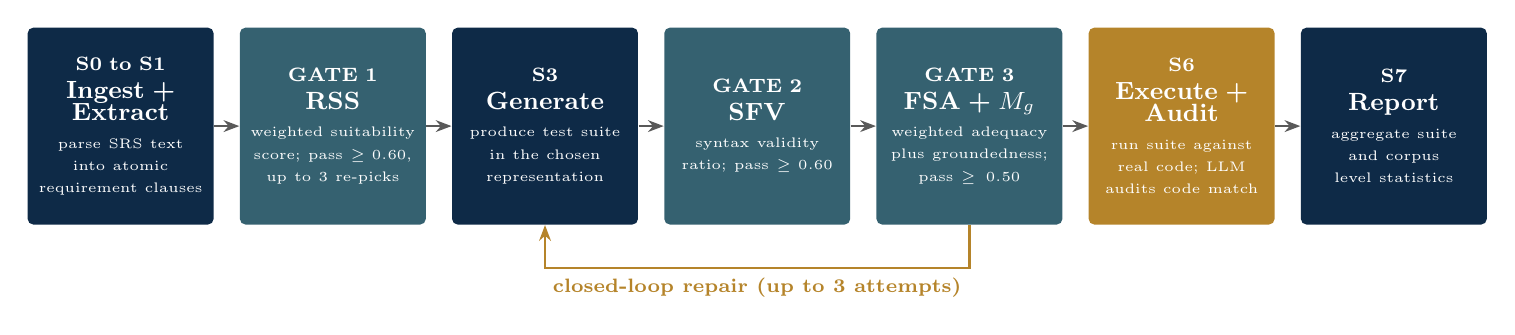
\begin{tikzpicture}[
  box/.style={rectangle, rounded corners=2pt, text=white, align=center,
    text width=2.15cm, minimum height=2.5cm, inner sep=3pt, font=\scriptsize},
  node distance=0.32cm
]
\node[box, fill=pnavy] (s01) {\textbf{S0 to S1}\\[2pt]{\small\textbf{Ingest +}}\\{\small\textbf{Extract}}\\[2pt]\tiny parse SRS text into atomic requirement clauses};
\node[box, fill=pteal, right=of s01] (g1) {\textbf{GATE 1}\\[2pt]{\small\textbf{RSS}}\\[2pt]\tiny weighted suitability score; pass $\geq 0.60$, up to 3 re-picks};
\node[box, fill=pnavy, right=of g1] (s3) {\textbf{S3}\\[2pt]{\small\textbf{Generate}}\\[2pt]\tiny produce test suite in the chosen representation};
\node[box, fill=pteal, right=of s3] (g2) {\textbf{GATE 2}\\[2pt]{\small\textbf{SFV}}\\[2pt]\tiny syntax validity ratio; pass $\geq 0.60$};
\node[box, fill=pteal, right=of g2] (g3) {\textbf{GATE 3}\\[2pt]{\small\textbf{FSA + $M_g$}}\\[2pt]\tiny weighted adequacy plus groundedness; pass $\geq 0.50$};
\node[box, fill=pgold, right=of g3] (s6) {\textbf{S6}\\[2pt]{\small\textbf{Execute +}}\\{\small\textbf{Audit}}\\[2pt]\tiny run suite against real code; LLM audits code match};
\node[box, fill=pnavy, right=of s6] (s7) {\textbf{S7}\\[2pt]{\small\textbf{Report}}\\[2pt]\tiny aggregate suite and corpus level statistics};

\foreach \a/\b in {s01/g1, g1/s3, s3/g2, g2/g3, g3/s6, s6/s7}
  \draw[-{Stealth[length=2mm]}, thick, gray!70!black] (\a.east) -- (\b.west);

\coordinate (dropg3) at ($(g3.south)+(0,-0.55cm)$);
\coordinate (drops3) at ($(s3.south)+(0,-0.55cm)$);
\draw[-{Stealth[length=2mm]}, thick, pgold] (g3.south) -- (dropg3) -- (drops3) -- (s3.south);
\node[below, font=\scriptsize\bfseries, text=pgold] at ($(dropg3)!0.5!(drops3)$) {closed-loop repair (up to 3 attempts)};
\end{tikzpicture}
\caption{The requirement-to-test pipeline: extraction, the three gates in
sequence with their exact formulas and thresholds as implemented, closed-loop
repair on Gate-3 failure, then execution/audit against the real
implementation.}
\label{fig:pipeline}
\end{figure*}

We note, as a methodological point, that two earlier design documents
produced during this project specify different thresholds for Gates 2 and 3
(SFV $\geq 0.80$, FSA $\geq 0.75$) and a simpler four-term FSA without
groundedness. The numbers above are not those design-document values; they
are what the pipeline implementation actually enforced when producing every
result in this paper, confirmed directly against the configuration module.
We flag the discrepancy explicitly because a methods section that quietly
followed the more demanding, unimplemented thresholds would misrepresent the
very results it reports, an error of exactly the kind this paper is
arguing the field should stop making silently.

\subsection{Prompt Design}
\label{sec:prompts}
Every prompt used in the pipeline is a plain text template with explicit
placeholders, stored and versioned separately from the pipeline code, so that
what a model was actually asked is always directly inspectable rather than
reconstructed from code. Table~\ref{tab:prompts} gives the abbreviated form of
the three prompts most central to this paper's argument: the representation
choice prompt (Gate 1), the generation prompt (Stage S3), and the judge
prompt (Gate 3). Full prompt text is included in the project repository.

\begin{table*}[t]
\centering
\caption{Abbreviated prompt templates for the stages central to this paper (placeholders shown as \texttt{\{\{FIELD\}\}})}
\label{tab:prompts}
\small
\begin{tabular}{@{}p{0.17\linewidth}p{0.17\linewidth}p{0.61\linewidth}@{}}
\toprule
\textbf{Prompt} & \textbf{Used at} & \textbf{Abbreviated template} \\
\midrule
\texttt{select\_reps.txt} & Gate 1 (representation choice) &
\texttt{"Choose the test-case representations best suited to the requirements below.} \newline
\texttt{REQUIREMENTS: \{\{REQS\}\}\ \ DEPENDENCIES: \{\{DEPS\}\}\ \ AVAILABLE REPRESENTATIONS: \{\{CATALOG\}\}} \newline
\texttt{Pick the \{\{K\}\} most suitable, judged by concern alignment, abstraction level, simplicity, and LLM feasibility.} \newline
\texttt{Respond with ONLY a JSON object: \{"selected": [\{"representation": ..., "covers": [...], "reason": ...\}]\}"} \\
\addlinespace
\texttt{generate.txt} & Stage S3 (test generation) &
\texttt{"Write a complete test suite for the requirements below in the representation \{\{REP\}\}.} \newline
\texttt{REQUIREMENTS: \{\{REQS\}\}\ \ DEPENDENCIES (context only): \{\{DEPS\}\}\ \ SUFFICIENCY CRITERIA: \{\{CHECKLIST\}\}} \newline
\texttt{The suite will be scored on: syntactic validity; clause coverage; negative and boundary paths; oracle assertiveness; groundedness (every concrete value must come from the requirement text, never invented).} \newline
\texttt{Output exactly two fenced blocks: the artifact in \{\{REP\}\} notation, and the same cases as canonical JSON."} \\
\addlinespace
\texttt{fsa\_judge.txt} & Gate 3 (semantic adequacy judge) &
\texttt{"You are an independent test-quality evaluator. You did NOT write the suite below. Score it strictly against the SRS requirements, and check every concrete value for hallucination.} \newline
\texttt{REQUIREMENTS (ground truth): \{\{REQS\}\}\ \ ARTIFACT: \{\{ARTIFACT\}\}\ \ CANONICAL CASES: \{\{TESTCASES\}\}} \newline
\texttt{Score clause\_coverage, negative\_coverage, oracle\_assertiveness, boundary\_coverage in [0,1]; for every concrete element asserted, decide "grounded": true/false by entailment against the SRS text.} \newline
\texttt{Respond with ONLY a JSON object: \{"clause\_coverage": ..., ..., "concrete\_elements": [\{"value": ..., "grounded": ...\}], "weaknesses": [...]\}"} \\
\bottomrule
\end{tabular}
\end{table*}

The judge prompt (\texttt{fsa\_judge.txt}) is the one most relevant to
Section~\ref{sec:validity}: it instructs the judge to decide, value by value,
whether a concrete number, name, or state asserted in the suite is actually
entailed by the requirement text, which is exactly the groundedness check
later found to disagree so often with what execution against real code shows.

\section{Experimental Setup}
\label{sec:setup}

\subsection{Model Selection}
Candidate models were narrowed from an initial pool of 65 through a
four-stage funnel: licensing/recency screening (65$\rightarrow$31$\rightarrow$29),
hardware feasibility by VRAM and context length (29$\rightarrow$22), capability
and benchmark screening (22$\rightarrow$16), and a final state-of-the-art
(SOTA)/diversity pass
(16$\rightarrow$14), yielding 12 open-weight models plus two closed-source
controls (GPT-4o, Claude 3.5 Sonnet) intended as reference points.

Of the 12 open-weight models, \textbf{10 completed the full benchmark}:
Llama-3.1-8B, Qwen2.5-Coder-7B, Qwen2.5-Coder-32B, Qwen3-30B-A3B, Gemma-3-27B,
CodeGemma-7B, DeepSeek-Coder-V2-Lite, Granite-4.1-8B, Phi-3.5-mini, and
Phi-3.5-MoE. Phi-4-14B failed Gate 1 on every attempted unit (server errors
mid-generation) and is excluded from the comparative results; Llama-3.3-70B
and the two closed-source controls were not executed, for compute and cost
reasons. We also note that Gemma-3-27B and DeepSeek-Coder-V2-Lite completed
only a small fraction of the full unit set (7 and 6 suites respectively,
against 58 to 61 for the other eight models); their aggregate statistics
below should be read with correspondingly lower confidence.

\subsection{Case Studies}
Three SRS/implementation pairs were used, each with its generated tests later
compared against its real codebase (Section~\ref{sec:results}):
\begin{itemize}
\item \textbf{doorstop}: the requirements-management tool Doorstop, with
its own Python implementation. 13 requirements extracted; time-budgeting
restricted generation to 2 units, each run against 2 representations
(4 suites per model).
\item \textbf{ventilator}: an open-source ventilator control system with
its own SRS and software implementation. 151 requirements extracted; 21
units generated, one representation per unit.
\item \textbf{virtual\_clinic}: a clinic-management web application
(Django-based) with a PDF SRS. 251 requirements extracted; 36 units
generated, one representation per unit.
\end{itemize}
Across the three case studies and 10 executed models this yields
\textbf{496 test suites and 4{,}058 test cases} (40 doorstop, 170 ventilator,
286 virtual\_clinic suites). The same extraction, judge, and executor model
(\texttt{gpt-oss-20b}, a different model family from every subject under
test) was used for every generator, to avoid a model favouring its own
family's outputs. Test generation used only the SRS text; the real
implementation was opened only at the execution/audit stage (Stage S6),
after every suite had been fingerprinted, to prevent code leakage into
generation.

\section{Results I: Model and Representation Comparison}
\label{sec:results}

\begin{table}[t]
\centering
\caption{Mean adequacy by model, doorstop case study (same units for every
model; $n=4$ suites/model). G2 and G3 are the Gate 2 (SFV) and Gate 3 (FSA)
pass rates; ``both'' is the share of suites passing both gates.}
\label{tab:doorstop}
\small
\begin{tabular}{@{}lrrrr@{}}
\toprule
Model & G2 pass & G3 pass & both & FSA \\
\midrule
Llama-3.1-8B & 100\% & 100\% & 100\% & 0.73 \\
Qwen2.5-Coder-32B & 75\% & 75\% & 75\% & 0.67 \\
Gemma-3-27B & 100\% & 100\% & 100\% & 0.66 \\
DeepSeek-Coder-V2-Lite & 75\% & 25\% & 25\% & 0.63 \\
Granite-4.1-8B & 75\% & 50\% & 50\% & 0.57 \\
Qwen2.5-Coder-7B & 50\% & 50\% & 50\% & 0.55 \\
Qwen3-30B-A3B & 25\% & 25\% & 25\% & 0.53 \\
Phi-3.5-MoE & 25\% & 25\% & 25\% & 0.53 \\
CodeGemma-7B & 75\% & 25\% & 25\% & 0.47 \\
Phi-3.5-mini & 0\% & 0\% & 0\% & n/a \\
\bottomrule
\end{tabular}
\end{table}

Fig.~\ref{fig:fsa-model} shows mean FSA per model pooled across all three
case studies. We emphasize a reading hazard visible in this figure: mean FSA
is computed only over suites that \emph{reached} the judge (\ie passed
Gate 2), so a model with a very low Gate-2 pass rate can still show a high
mean FSA on the small number of suites it did get judged on. Phi-3.5-mini,
for instance, shows the single highest pooled mean FSA (0.74) in
Fig.~\ref{fig:fsa-model} despite passing Gate 2 on only 9\% of its 58
attempted suites and Gate 3 on only 2\%; a leaderboard built from FSA
alone would rank it first on the strength of essentially one or two judged
suites. On the richer, equal-sample doorstop comparison (Table~\ref{tab:doorstop},
where every model attempted the same four suites), Llama-3.1-8B is the
clearest overall performer (FSA 0.73, both-gates 100\%) and CodeGemma-7B the
weakest among models that passed Gate 1 at all (FSA 0.47, both-gates 25\%).

\begin{figure*}[t]
\centering
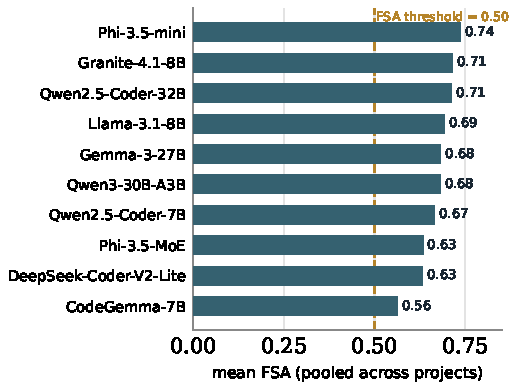
\includegraphics[width=\textwidth]{fig/fsa_by_model.pdf}
\caption{Mean FSA per model, pooled across all three case studies, with the
number of judged suites each mean is computed over. Sample sizes vary sharply
by model (6 to 61 judged suites); see text for why this figure alone should
not be read as a leaderboard.}
\label{fig:fsa-model}
\end{figure*}

Two comparisons that a practitioner might expect to predict quality do not:
model size (Spearman $\rho(\text{parameters}, \text{FSA})=-0.015$, $n=311$)
and code specialization (FSA 0.58 for code-specialized models vs.\ 0.64 for
general-purpose, Mann-Whitney $p=0.1407$). Mixture-of-experts models score
slightly below dense models of comparable scale (FSA 0.59 vs.\ 0.62).

Representation choice shows a larger, more consistent effect than model
identity. Fig.~\ref{fig:fsa-repr} breaks FSA and both-gates pass rate down by
the six paradigms of Section~\ref{sec:taxonomy}: Logical/Combinatorial
representations (decision tables, \etc) both score highest on mean FSA (0.70)
and pass both gates most often (55\%), while Stateful/Transitions
representations (FSMs, statecharts) are both lowest on FSA (0.62) and
both-gates pass rate (23\%). At the level of individual representations, the
30 available forms are used very unevenly: five representations (Gherkin,
xUnit, Use-Cases, Decision Tables, FSMs) account for the overwhelming
majority of all choices models made, with 18 of the 30 catalog
representations used at all. Strikingly, a model's own Gate-1 choice agrees
with the independent RSS heuristic's top-3 recommendation only 20\% of the
time on average; the two notions of ``suitable representation'' mostly
disagree, a point we return to in Section~\ref{sec:validity}.

Table~\ref{tab:byrepr} breaks this down to the level of individual
representations with at least 15 suites generated in that form. GUI Event
Graphs post the highest both-gates pass rate (64\%, $n=28$) despite a mid-pack
FSA; Decision Tables and Gherkin, the two most heavily-used representations,
sit in the middle; UML Testing Profile and Use-Cases \& User Stories, despite
very high syntactic validity (SFV 0.92 and 0.86), both-gates pass at only
27\% to 28\%, since most of their failures occur at the semantic Gate 3 rather
than the syntactic Gate 2, a reminder that a well-formed suite is not
automatically an adequate one.

\begin{table}[t]
\centering
\caption{Gate outcomes by representation ($n \geq 15$ suites; $n$ = suites
generated in that representation; ``both-pass'' = share passing both
Gate 2 and Gate 3)}
\label{tab:byrepr}
\small
\begin{tabular}{@{}lrrrr@{}}
\toprule
Representation & $n$ & SFV & both-pass & FSA \\
\midrule
GUI Event Graphs & 28 & 0.96 & 64\% & 0.74 \\
Decision Tables & 44 & 0.77 & 55\% & 0.70 \\
Gherkin (BDD DSL) & 207 & 0.82 & 54\% & 0.67 \\
Sequence Diagrams & 18 & 0.85 & 44\% & 0.67 \\
Finite State Machines & 40 & 0.71 & 28\% & 0.66 \\
Use-Cases \& User Stories & 39 & 0.86 & 28\% & 0.62 \\
xUnit Test Cases & 79 & 0.61 & 29\% & 0.68 \\
UML Testing Profile (UTP) & 15 & 0.92 & 27\% & 0.58 \\
\bottomrule
\end{tabular}
\end{table}

\begin{figure*}[t]
\centering
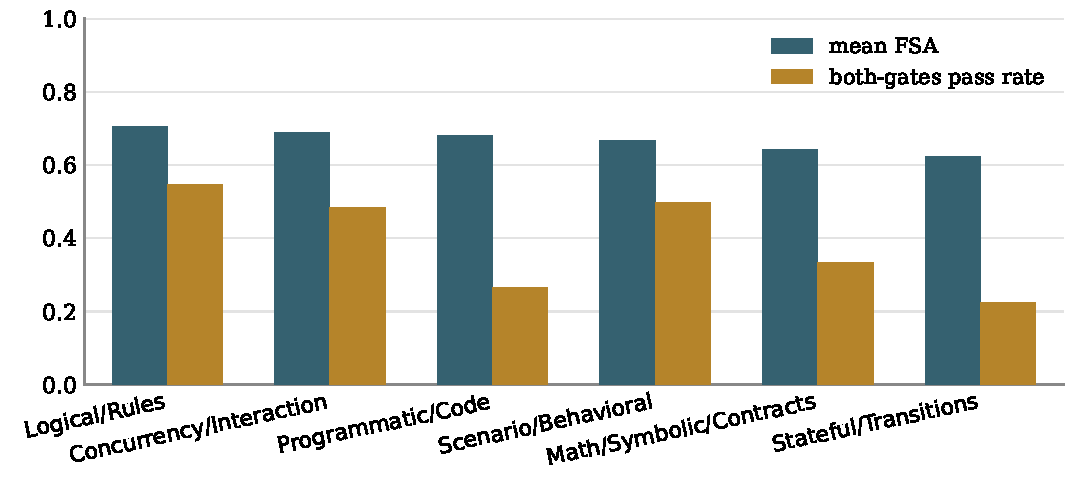
\includegraphics[width=\textwidth]{fig/fsa_by_repr_group.pdf}
\caption{Mean FSA and both-gates pass rate by representation paradigm, pooled
across all models and case studies.}
\label{fig:fsa-repr}
\end{figure*}

Closed-loop repair is effective where it is invoked: 207 of the 496 suites
were repaired after an initial Gate-3 failure, with a mean FSA gain of
$+0.131$ on those suites.

\section{Results II: Validity Checks}
\label{sec:validity}

Section~\ref{sec:results} reports what the three-gate pipeline says about
itself. This section checks those statements against evidence the pipeline
did not produce: real test execution, a code-grounded audit, and an
independent heuristic. All three checks were built into this study
specifically because we did not want to publish a benchmark leaderboard
without first asking how much the leaderboard's underlying scores can be
trusted.

\textbf{Execution agreement.} On doorstop, the one case study where generated
tests were actually executed against the real implementation rather than only
audited, the picture is stark: across the ten executed models, a combined
\textbf{148 generated tests for the eight best-represented models (and up to
315 when extended to the full 10-model doorstop run) produced only 1 to 2
passing executions in total}. Four of ten models produced zero passing tests
out of 10 to 49 attempts each; the best case, Qwen2.5-Coder-7B, passed 1 of 25.
Gate-passing and real test-execution success are, on this evidence, close to
unrelated for this case study: a suite that clears Gates 1 through 3 is not
meaningfully more likely to run successfully against the real system than one
that does not. The one weak positive signal is a moderate correlation between
FSA and execution pass rate across the models for which both are available
($\rho=0.433$, $n=15$), present but on a small sample, and far from
strong enough to license treating a high FSA score as evidence a suite will
execute correctly.

\textbf{Audit agreement.} Because full execution was only feasible for
doorstop (ventilator and virtual\_clinic lack an automatable test harness in
this study), the other two case studies instead rely on an LLM-judge
\emph{code audit}: the same judge model is shown retrieved code excerpts and
asked, for each test case, to return one of four verdicts describing whether
the code's behaviour matches the test's expectation: \texttt{satisfied}, the
code does what the test expects; \texttt{violated}, the code implements the
feature but disagrees with the expectation; \texttt{not\_implemented}, the
feature is absent; or \texttt{unclear}, the retrieved excerpt is insufficient
to tell. (On doorstop, actually running a test and seeing it fail triggers a
separate, three-way triage of \emph{why} it failed, by the same judge model:
\texttt{code\_mismatch}, the implementation disagrees with the requirement;
\texttt{test\_bug}, the generated test itself is wrong; or
\texttt{spec\_ambiguous}, the requirement does not clearly settle the
question.) On the subset of doorstop suites where both execution and audit
results are available ($n=11$), \textbf{the audit agrees with real execution
only 18\% of the time}. This is the single most important caveat on every
audit-based result reported for ventilator and virtual\_clinic elsewhere in
this paper and in the underlying analysis report: audit mode should be read
as a weak, frequently-wrong proxy for ground truth, not a substitute for
execution. Separately, across all three case studies, the audit flagged 190
individual test cases as contradicting the real implementation, combining an
audit \texttt{violated} verdict with, on the executed doorstop suites, an
execution-triage \texttt{code\_mismatch} verdict; given the 18\% agreement
rate just reported, this combined count should be treated as a rough signal
requiring manual confirmation, not a verified defect count.

\textbf{Representation-choice agreement.} As noted in
Section~\ref{sec:results}, a model's own Gate-1 pick of representation agrees
with the independent RSS heuristic's top-3 recommendation only 20\% of the
time on average. Gate 1 is designed to make representation choice
accountable to an external standard precisely because LLMs left to choose
freely cluster onto a handful of familiar notations
(Section~\ref{sec:results}); the low agreement rate shows that accountability
mechanism and the models' own judgment are, in practice, measuring different
things, and a high Gate-1 pass rate should not be read as confirmation that
the chosen representation was actually well suited to the requirement.

\textbf{Groundedness as a systematically missed failure mode.} 243 of 496
suites (49\%) assert at least one specific value (a timeout, a count, a
threshold) that cannot be traced back to the source requirement text (mean
6.1 hallucinated values per affected suite; mean groundedness $M_g=0.46$
across all judged suites). Because groundedness enters FSA as one of five
weighted components ($w_g=0.15$), a suite can still clear the FSA $\geq 0.50$
threshold while being substantially ungrounded, as long as its other four
components score well. We found 22 of 61 Gate-3-passing suites with
$M_g<0.5$ in a preliminary pass over the data, suites the pipeline reports
as adequate despite asserting more hallucinated values than grounded ones.

\textbf{Against the real implementation, directly.} Even setting execution
and audit reliability aside, the \emph{best-case} agreement between generated
tests and real requirement-level behaviour, measured as the share of SRS
requirements whose tests reach actually-implemented behaviour, is 54\%
(DeepSeek-Coder-V2-Lite, doorstop); the ceiling across every
model$\times$project pair in this study is just over half.

\textbf{Summary of Results I and II together.} The pipeline reports
both-gates pass rates of 25\% to 100\% depending on model and case study
(Table~\ref{tab:doorstop}), and a representation-paradigm effect that looks
like a clean, actionable signal (Fig.~\ref{fig:fsa-repr}). Set against real
execution, real code behaviour, and an independent heuristic, each of those
signals shrinks: 18\% audit-execution agreement, 1 to 2 passing tests out of
148 to 315 attempted, 20\% representation-choice agreement, and roughly half of
all suites carrying at least one hallucinated value. A three-gate, LLM-judged
pipeline is not nothing: it is more structured and more falsifiable than a
single similarity score, but on this evidence it is not yet a substitute
for execution-grounded validation, and should not be reported as one.

\section{Threats to Validity}
\label{sec:threats}

\textbf{Single run per configuration.} Every model$\times$unit$\times$
representation combination was run once at temperature 0; the underlying
analysis explicitly notes that differences of a few FSA points between models
are within expected noise and should not be over-interpreted.

\textbf{Single judge model.} All semantic adequacy, groundedness, and code
audit judgments were made by one model (\texttt{gpt-oss-20b}). We chose a
model from a different family than every subject under test to reduce
self-preference bias, a judge limitation documented in prior LLM-as-judge
work~\cite{zheng2023judging}, but we did not cross-validate its judgments against a
second judge model or human raters beyond the audit-vs-execution check in
Section~\ref{sec:validity}, which itself shows that judge's reliability is
limited.

\textbf{Uneven execution coverage.} Real test execution was only feasible for
doorstop; ventilator and virtual\_clinic results rely on the audit proxy,
which Section~\ref{sec:validity} shows agrees with execution only 18\% of the
time on the one case study where both are available. Conclusions drawn from
ventilator/virtual\_clinic audit data alone should be read as provisional.

\textbf{Partial model coverage.} Gemma-3-27B and DeepSeek-Coder-V2-Lite
completed only 6 to 7 suites each, against 58 to 61 for the other eight executed
models; Phi-4-14B failed to pass Gate 1 on any attempted unit; Llama-3.3-70B
and both closed-source controls (GPT-4o, Claude 3.5 Sonnet) were not
executed. The 10-model comparison in this paper is therefore narrower than
the 14-model selection funnel that produced it, and entirely open-weight.

\textbf{Three case studies.} doorstop, ventilator, and virtual\_clinic differ
in size and domain but are three systems; generalizing findings here to SRS
documents of very different style, domain, or scale (\eg safety-critical
avionics specifications) should be done cautiously.

\section{Discussion}

The clearest actionable finding from Section~\ref{sec:results} is that
\emph{which representation a requirement is tested with matters more than
which model generates the test}, a result consistent with the motivating
premise of this paper's own taxonomy (Section~\ref{sec:taxonomy}), and one
that argues for representation-aware tooling over simply swapping in a larger
or more code-specialized model.

The more consequential finding, from Section~\ref{sec:validity}, is that this
and plausibly other LLM-judge-based evaluation pipelines should not be
trusted to report correctness without an execution-grounded check built in
and reported alongside the gate scores. We did not find this gap by assuming
our framework was flawed; we found it by deliberately building the
cross-checks (execution comparison, code audit, independent heuristic) that a
pipeline reporting only its own gate scores would never surface on its own.
We think this is the more general lesson: any LLM-as-judge evaluation
pipeline for generated tests should report at least one such cross-check, not
only its own internal pass rates, and groundedness in particular is
well-suited to being promoted from a weighted component of a blended score to
an independently thresholded gate, given how cleanly it can hide inside a
passing FSA score (Section~\ref{sec:validity}).

\section{Related Work}

Prior work on automated test generation for requirements spans search-based
software testing (SBST) approaches, such as EvoSuite~\cite{fraser2011evosuite},
that evolve tests against coverage or mutation-based fitness functions
without needing a natural-language source, and, more recently, LLM-based
generation that consumes requirements or code directly. Roy~\etal~\cite{roy2024empirical} empirically study LLMs for unit
test generation and motivate much of the skepticism toward surface-similarity
metrics that this paper builds on. Reflexion-style self-feedback
loops~\cite{shinn2023reflexion} are methodologically close to this paper's
closed-loop repair step, though applied there to general agentic tasks rather
than test-suite adequacy specifically. SWE-bench and SWE-agent~\cite{jimenez2024swebench,wang2024sweagent}
establish benchmark-and-agent pairs for a different software-engineering task
(issue resolution) but share this paper's concern with evaluating an LLM's
output against a real, executable ground truth rather than a static
reference. Model licensing and openness considerations in our Section~\ref{sec:setup}
model-selection funnel draw on the evaluation framework of
Luccioni~\etal~\cite{luccioni2023openness}; the open-weight code models in
our benchmark are drawn from model families documented in
\cite{li2023starcoder,deepseek2024coderv2}, with general LLM behaviour and
instruction-tuning background from \cite{chen2023chatgpt,ouyang2022instructgpt}.

\section{Conclusion}

We set out to build a careful, multi-gate alternative to text-similarity
metrics for evaluating LLM-generated, requirement-derived test suites, and
benchmarked it across 10 models and three real SRS/implementation pairs. The
resulting comparative findings, that model size and code specialization do
not predict adequacy while representation choice does, are useful on their
own. But the paper's central result is that the pipeline's own gate-passing,
checked against real execution, a code audit, and an independent heuristic,
agrees with ground truth far less often than its pass rates alone would
suggest. We report this as a finding about the field's current direction, not
only about our own pipeline: as LLM-as-judge evaluation becomes the default
replacement for text-similarity metrics in test generation research, it needs
to be held to the same standard it was introduced to meet, with
execution-grounded validity checks reported as a matter of course rather than
as an afterthought.

\section{Planned Changes}
\label{sec:future}

Table~\ref{tab:gaps} collects, in one place, every validity gap this paper
measured and the specific change we plan to make in response to it. Each row
names the evidence (already reported in Section~\ref{sec:validity}) rather
than repeating it, so this table should be read as a punch list rather than a
new set of claims.

\begin{table*}[t]
\centering
\caption{Every validity gap measured in this paper, and the planned change addressing it}
\label{tab:gaps}
\small
\begin{tabular}{@{}p{0.27\linewidth}p{0.33\linewidth}p{0.33\linewidth}@{}}
\toprule
\textbf{Gap} & \textbf{Evidence (Section~\ref{sec:validity})} & \textbf{Planned change} \\
\midrule
Gate-passing does not predict execution success & 1 to 2 of 148 to 315 generated doorstop tests actually pass; $\rho=0.433$ between FSA and execution pass rate, $n=15$ &
Report an execution-grounded pass rate alongside every gate score, not only on doorstop (see ``Full Execution Coverage'' below) \\
\addlinespace
Code audit is an unreliable stand-in for execution & Audit agrees with real execution only 18\% of the time ($n=11$) &
Replace audit-only results for ventilator and virtual\_clinic with real execution, and report audit-execution agreement per project rather than assuming it transfers \\
\addlinespace
Representation choice is not accountable to an external standard & Model's own Gate-1 pick agrees with the independent RSS heuristic's top-3 only 20\% of the time &
Formalize explicit dependency-type-to-representation mapping rules (see ``Representation Mapping Rules'' below) rather than leaving the mapping heuristic \\
\addlinespace
Groundedness can hide inside a passing adequacy score & 243 of 496 suites (49\%) assert an ungrounded value; 22 of 61 Gate-3-passing suites have $M_g<0.5$ &
Promote groundedness from a weighted FSA component to its own independently thresholded gate \\
\addlinespace
Evaluation stops at a single requirement unit & Every suite in this study covers one unit of up to 8 requirements in isolation; no end-to-end, interaction, failure, or quality-attribute coverage is measured &
Extend the framework to system-level testing with an explicit, multi-dimensional coverage denominator (see ``System-Level Test Generation'' below) \\
\bottomrule
\end{tabular}
\end{table*}

\subsection{Representation Mapping Rules}
The 20\% agreement between a model's free Gate-1 choice and the independent
RSS heuristic (Section~\ref{sec:validity}) shows the two views of
``suitable representation'' are, at present, only loosely connected. We plan
to formalize explicit mapping rules from requirement dependency type (state,
interaction, data, concurrency, as used in the RSS heuristic itself) to a
short ranked list of representations, so that representation selection is
governed by a documented, inspectable rule set rather than left to either an
LLM's free choice or a keyword heuristic alone.

\subsection{Full Execution Coverage}
Real execution in this study was only feasible for doorstop; ventilator and
virtual\_clinic results rely on the weaker audit proxy, which
Section~\ref{sec:validity} shows agrees with execution only 18\% of the time
on the one case study where both are available. The next iteration of this
work builds an automatable execution harness for both remaining case studies,
so that the 18\% audit-execution agreement figure can either be confirmed as
a general property of this evaluation approach or shown to be specific to
doorstop.

\subsection{System-Level Test Generation}
\label{sec:sysleveltesting}
Every suite reported in this paper covers exactly one requirement unit, up to
8 requirements drawn from a single SRS section, in isolation. Nothing in the
current framework exercises a flow that spans multiple units, a dependency
between two separately specified requirements, an environment or component
failure, or a quality attribute (latency, throughput, reliability) that only
manifests across the running system rather than inside one function. Closing
this gap is the most structurally different piece of planned work, since it
requires a ground-truth structure the current unit-level canonical schema
(Section~\ref{sec:framework}) does not provide: an explicit coverage
denominator at the system level, analogous to what traceability already gives
at the unit level.

We are evaluating two candidate ground-truth formats for this purpose, shown
in Fig.~\ref{fig:sysgt} and summarized below.

\begin{figure*}[t]
\centering
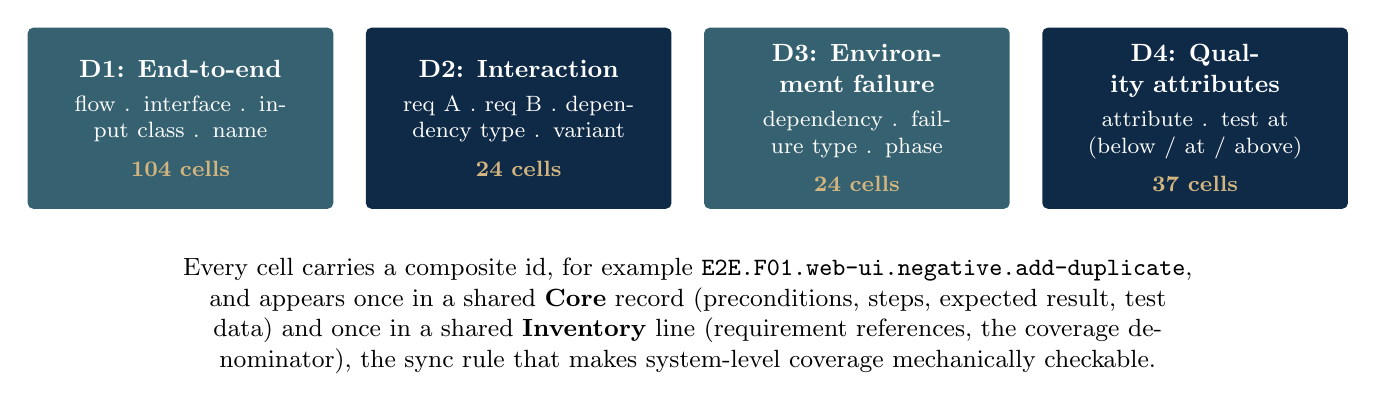
\begin{tikzpicture}[
  dimbox/.style={rectangle, rounded corners=2pt, text=white, align=center,
    text width=3.6cm, minimum height=2.3cm, inner sep=4pt, font=\small},
  node distance=0.4cm
]
\node[dimbox, fill=pteal] (d1) {\textbf{D1: End-to-end}\\[3pt]\footnotesize flow . interface . input class . name\\[3pt]\textcolor{pgold!60!white}{\textbf{104 cells}}};
\node[dimbox, fill=pnavy, right=of d1] (d2) {\textbf{D2: Interaction}\\[3pt]\footnotesize req A . req B . dependency type . variant\\[3pt]\textcolor{pgold!60!white}{\textbf{24 cells}}};
\node[dimbox, fill=pteal, right=of d2] (d3) {\textbf{D3: Environment failure}\\[3pt]\footnotesize dependency . failure type . phase\\[3pt]\textcolor{pgold!60!white}{\textbf{24 cells}}};
\node[dimbox, fill=pnavy, right=of d3] (d4) {\textbf{D4: Quality attributes}\\[3pt]\footnotesize attribute . test at (below / at / above)\\[3pt]\textcolor{pgold!60!white}{\textbf{37 cells}}};
\coordinate (rowmid) at ($(d1.south)!0.5!(d4.south)$);
\node[below=0.5cm of rowmid, font=\small, text width=15.5cm, align=center] (inv)
  {Every cell carries a composite id, for example \texttt{E2E.F01.web-ui.negative.add-duplicate},
  and appears once in a shared \textbf{Core} record (preconditions, steps, expected result, test data)
  and once in a shared \textbf{Inventory} line (requirement references, the coverage denominator),
  the sync rule that makes system-level coverage mechanically checkable.};
\end{tikzpicture}
\caption{The four coverage dimensions of the structured ground-truth
candidate for planned system-level testing (Section~\ref{sec:sysleveltesting}),
with the pilot inventory's cell count per dimension (189 cells total).}
\label{fig:sysgt}
\end{figure*}

\textbf{Candidate 1: a structured, dimension-based schema.} Every test is one
cell addressed by a composite id, for example
\texttt{E2E.F01.web-ui.negative.add-duplicate}, decomposing into a flow, an
interface, an input class, and a name. Each cell appears in three places: a
core record (preconditions, steps with an expected result per step, test
data), a dimension-specific record (one of D1 end-to-end, D2 interaction
between two requirements, D3 environment or component failure, or D4 a
quality attribute tested below, at, or above its threshold), and an inventory
line carrying the requirement references that cell covers. A sync rule, every
cell id appears exactly once in the core, once in its dimension, and once in
the inventory, makes system-level coverage mechanically checkable the same
way unit-level traceability already is in this paper's framework (a pilot
inventory built this way holds 189 cells across the four dimensions).

\textbf{Candidate 2: an industrial, spreadsheet-style sheet.} A simpler
alternative closer to common ISO/IEC/IEEE 29119 (the international software
testing standard) style test-case documentation:
one row per test, with id, name, requirement links, precondition, steps,
expected result, postcondition, and use case as columns, plus a separate
methodology sheet classifying each row as happy-path, negative, or boundary.
This format is easier for a human reviewer to read and already separates
expected result from postcondition, but it has no explicit coverage-item
inventory or denominator, so system-level coverage cannot be computed from it
the way it can from Candidate 1, and concrete test-data values are more often
left as vague placeholders.

We plan to pilot Candidate 1 first, since its explicit, checkable denominator
extends this paper's existing traceability methodology most directly from the
unit level to the system level, and to compare it against Candidate 2 on
reviewer readability and on whether the heavier structure measurably improves
coverage auditability in practice before committing to either format for the
full benchmark.

\section*{Data and Code Availability}
The pipeline, prompts, gate implementation, aggregated results
(\texttt{suites.csv}, the analysis report), and this paper's own source are
published at \url{https://github.com/poojitha376sp/Clean_exp}. The planned
system-level ground-truth templates discussed in
Section~\ref{sec:sysleveltesting} are tracked in the same repository under
\texttt{paper/}.

\begin{thebibliography}{00}
\bibitem{chen2023chatgpt} L. Chen, M. Chen, and J. Zou, ``How is ChatGPT's Behavior Changing Over Time?'' arXiv preprint arXiv:2307.09009, 2023.
\bibitem{ouyang2022instructgpt} L. Ouyang et al., ``Training language models to follow instructions with human feedback,'' Advances in Neural Information Processing Systems, vol. 35, pp. 27730--27744, 2022.
\bibitem{roy2024empirical} S. Roy et al., ``An Empirical Study of Large Language Models for Unit Test Generation,'' IEEE Transactions on Software Engineering, 2024.
\bibitem{jimenez2024swebench} C. E. Jimenez et al., ``SWE-bench: Can Language Models Resolve Real-World GitHub Issues?'' ICLR 2024.
\bibitem{luccioni2023openness} A. Luccioni et al., ``A Framework for Evaluating the Openness and Licensing of Foundation Models,'' arXiv preprint arXiv:2309.05678, 2023.
\bibitem{li2023starcoder} R. Li et al., ``StarCoder: May the source be with you!'' ACM Transactions on Computer-Human Interaction, 2023.
\bibitem{wang2024sweagent} J. Wang et al., ``SWE-agent: Agent-Computer Interfaces Enable LLMs to Resolve Software Engineering Issues,'' arXiv preprint arXiv:2405.15793, 2024.
\bibitem{shinn2023reflexion} N. Shinn et al., ``Reflexion: Language Agents with Systematic Self-Feedback,'' NeurIPS 2023.
\bibitem{deepseek2024coderv2} DeepSeek-AI, ``DeepSeek-Coder-V2: Breaking the Barrier of Closed-Source Models in Code Intelligence,'' arXiv preprint arXiv:2406.11931, 2024.
\bibitem{fraser2011evosuite} G. Fraser and A. Arcuri, ``EvoSuite: Automatic Test Suite Generation for Object-Oriented Software,'' in Proc. 19th ACM SIGSOFT Symp. and 13th European Conf. on Foundations of Software Engineering (ESEC/FSE), 2011. DOI: 10.1145/2025113.2025179.
\bibitem{zheng2023judging} L. Zheng et al., ``Judging LLM-as-a-Judge with MT-Bench and Chatbot Arena,'' arXiv preprint arXiv:2306.05685, 2023.
\end{thebibliography}

\end{document}
